\section{Nvidia GPUs architecture and CUDA}\label{C2}
Scientists, years by years, face bigger and bigger problems. 
Even if Moore's law (that said: "the number of transistors in an integrated circuit double about every two years") determines the increased power of the CPU since the sixties, even the problems size grows and it grows also much more quickly. For example, the web growth since the turn of the millennium raises new challenges that are hard to solve with standard algorithms.  \\
Besides, at the same time, the manufacturers face some serious physical limits. The increase in performance was made possible by the reduction in the size of the transistors and the increase in the frequency of the clock cycle. In the first half of the first decade of 2000, the producers discovered that reducing, even more, the size causes serious problems of heat dissipation and data synchronization. To find a solution to this problems, the manufactures start to produce multi-core CPUs: the idea is that if it's impossible to increase further the speed with only one core, they add another processing unit, to ideally halve the execution time.\\
For these reasons, in recent times the studies of new parallel approaches became fundamental to solve problems that can not be solved classically. As a result of this change and at the same time both the support of floating-point number on the graphics processing units (GPU) and the advent of programmable shaders, it became popular the general-purpose computing on GPU (GPGPU), i.e. the use of a GPU to perform a computation that is commonly handled by the CPU.\\
\begin{figure}[h]
	\centering
	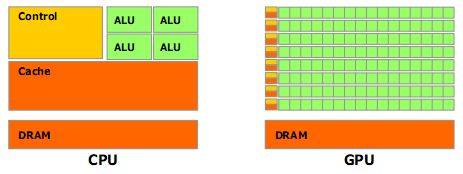
\includegraphics[width=0.7\linewidth]{0-resources/cpugpuhardware}
	\caption{Difference in CPUs and GPUs architecture. This image was reprinted from \cite{cuda_manual} }
	\label{fig:cpugpuhardware}
\end{figure}
\\
The GPU architecture is radically different respect to the CPU. The CPU has several ALUs (Arithmetic and Logic Unit), a complex control unit that controls those ALUs, big fast cache memory and dynamic random access memory (DRAM); the GPU has many ALUs, several simple control units, a smaller cache and a DRAM (Figure \ref{fig:cpugpuhardware}). While the first one is focused on the low-latency, the second one is focused on the high throughput;
while the first one is focused on handle various serial complex instruction, the second is focused on handle much parallel simple instruction.
In brief, the first one is a versatile processing unit, the second one is highly specialized.
Even if in recent time the multi-core CPU performance get closer to the performance of the GPU \cite{gpucpu}, from the Figure \ref{fig:cpugpu} we can see how the performance of the GPU outclasses the performance on the CPU.\\
\begin{figure}[h]
	\centering
	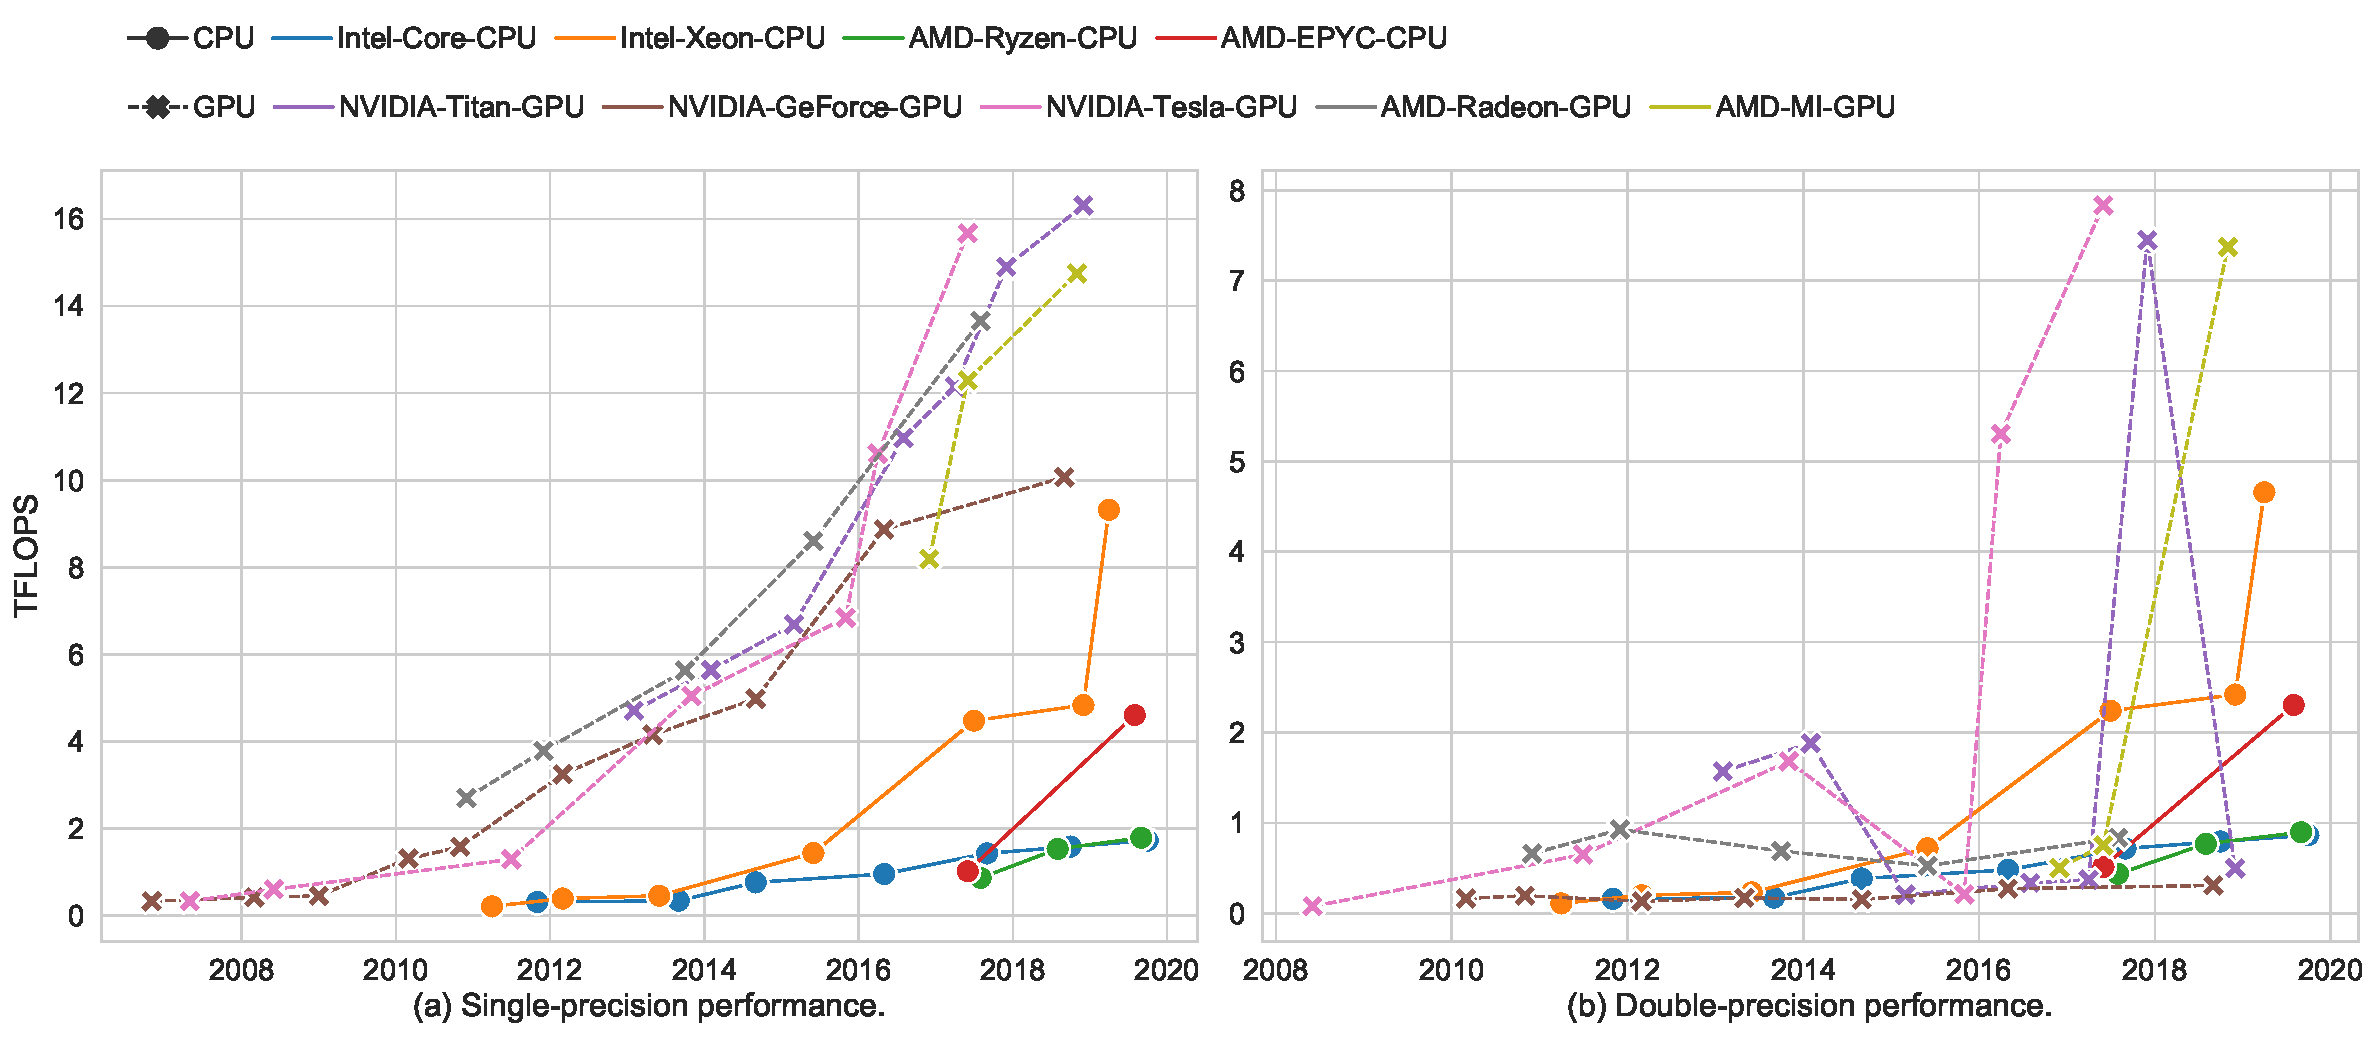
\includegraphics[width=1.\linewidth]{0-resources/cpu_gpu}
	\caption{Comparing single-precision and double-precision performance of CPUs and GPUs. The performance are measured in trillion of floating point operations per Second (TFLOPS). This image was reprinted from \cite{gpucpu}.}
	\label{fig:cpugpu}
\end{figure} 
\\	
For those reasons, the GPU-accelerated applications are the most effective to solve big problems, due to the possibility of reach very high speed-up compared to the classic multi-core applications. 
To simplify the development of this type of applications, in 2007, Nvidia releases CUDA (Compute Unified Device Architecture), a parallel computing platform and application programming interface model.
Nowadays, the CUDA framework is one of the main tools to develop HPC applications, due to its performance and simple API, and for this, we choose to use it in this project.
In this chapter, we first present the Nvidia's GPU architecture, then we present CUDA and Thrust, a parallel computing library. This chapter was based on \cite{turing} and \cite{cuda_manual}.
\subsection{Nvidia's GPU Architecture}
We present Nvidia's GPU Architecture to introduce some key concepts that are used later in the thesis. This introduction presents the Nvidia Turing architecture, which is the latest released. We present the highest performing GPU of the Turing line, The Turing TU102 GPU (Turing machine can be also scaled-down from this one). 
In Figure (\ref{fig:tuning:a}) we can see a scheme of this architecture.
\begin{figure}[h]\label{fig:tuning}
	\hspace*{-4em}
	\subcaptionbox{\label{fig:tuning:a}}{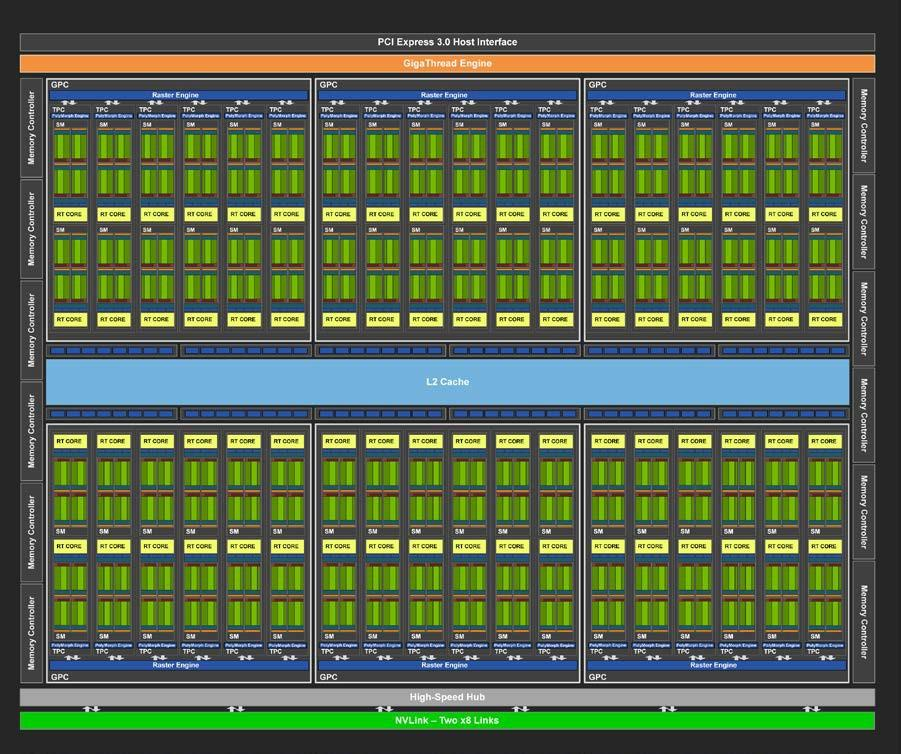
\includegraphics[width=0.72\linewidth]{0-resources/turing}}\hspace{4em}%
	\subcaptionbox{\label{fig:tuning:b}}{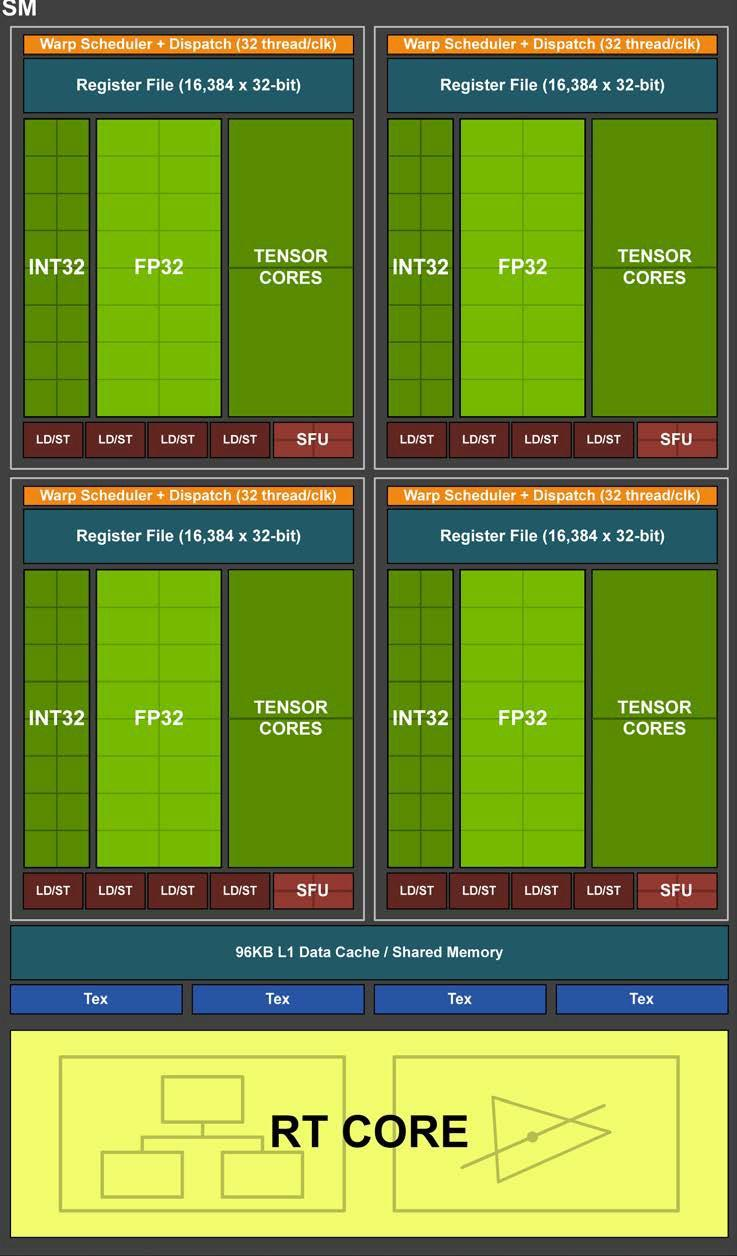
\includegraphics[width=0.4\linewidth]{0-resources/sm}}
	\caption{(a): Tuning GPU full architecture; (b) Streaming multiprocessor (SM) in details. Those images was reprinted from \cite{turing} }
\end{figure}
The cornerstone of each Nvidia's GPU is the concept of Streaming Multiprocessor (SM), that are represented\\in Figure (\ref{fig:tuning:b}): it contains some cores specialised to solve specific arithmetic operations on specific types of data (like integer, float, double, tensor...).
In a Tuning machine, each SM contains 64 FP32 cores, 64 INT32 cores, eight Tensor cores and two FP64 cores (that aren't present in Figure \ref{fig:tuning:b}). In Turing architecture is present also a Ray Tracing cores in each SMs: this core is used in rendering.\\
The SM is the fundamental unit because the parallel execution of the code in a CUDA application it's organized in blocks, and each block is executed on a single SM. 
Moreover, the SM contains also some registers (256 KB in Turing), an L1 cache and a shared memory (in Turing 96 KB of L1/shared memory which can be configured for various capacities). 
The multiprocessor creates, manages, schedules, and executes threads in groups of
32 parallel threads called warps: when we give one or more thread blocks to execute to a a streaming multiprocessor, it partitions them into warps that get scheduled by a warp scheduler to be executed. 
A very important notion is that each warp executes one common instruction at a time, so if threads of a warp diverge via a conditional branch, the warp serially executes each branch path taken, ignoring the instruction for the threads that are not on the active path. 
The registers are private for each thread, but all threads share the SM's shared memory.\\
The SMs are organised in Texture Processing Clusters (TPCs), that in a Turing GPU contains two SMs.
In their turn, the TPCs are organized in Graphics Processing Clusters (GPC) that in a TU102 contains six TPCs. Finally, each GPU's contain six GPCs. Shared between all components, there is a shared L2 cache, i.e. each thread can have access to it. In the Turing GP, it is large 6144 KB.
Therefore, in summary, a Turing TU102 GPU contains 72 SMs and 4608 FP32 cores, 4608 INT32 cores, 576 tensor core and 144 FP64 cores.

\subsection{CUDA}
In November 2006, CUDA (that stands for Compute Unified Device Architecture) was realised by NVIDIA. This general-purpose parallel computing interface aims at providing a framework to the developers that allow building applications that can transparently scale with a low learning curve. To overcome this challenge, CUDA was designed as a C++ language extension: in this way, a programmer that already knows the language syntax can start to develop a GPU-accelerated application with a minimal effort. The support of other language was introduced years by years, as illustrated in Figure \ref{fig:gpu-computing-applications}. In this chapter we present the C++ extension, that was used to develop the project illustrated in this thesis, even if all extensions share the same concept and programming model.
\begin{figure}
	\centering
	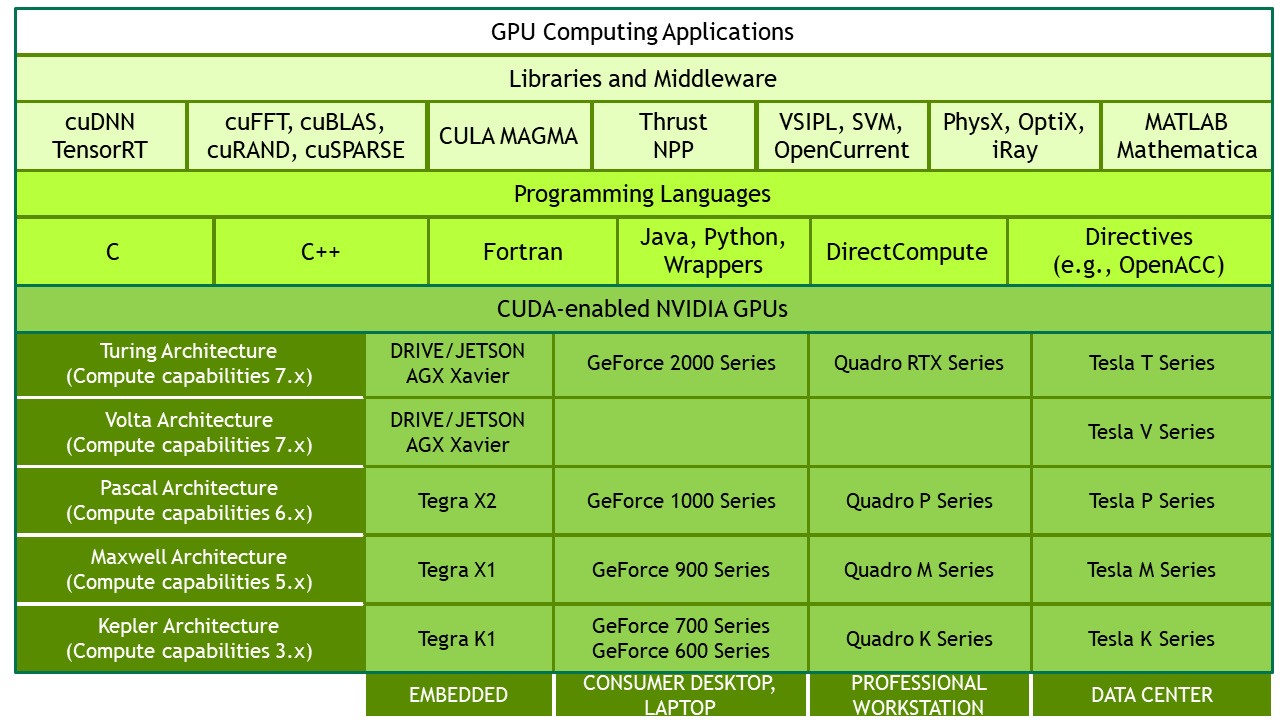
\includegraphics[width=0.8\linewidth]{0-resources/gpu-computing-applications}
	\caption{GPU Computing Applications. This image was reprinted from \cite{cuda_manual}.}
	\label{fig:gpu-computing-applications}
\end{figure}\\
The first key concept is the \textbf{kernel} function. In a CUDA-based application we define as \textbf{device} the GPU and as \textbf{host} the CPU. The application starts at the host, and when it is needed, it calls a kernel function that executes the function $n$ times in parallel by $n$ different threads. To define a kernel, we have to add \verb|__global__| declaration specifier to the method and the number of threads that have to execute the kernel call. Each thread has a unique ID. To set the thread number we use an execution configuration syntax: after the method name, we include this setup enclosed in three angle brackets \verb|<<< ... >>>|. The configuration is used to define the number and the size of the blocks: a block is a group of threads that are organized in a one, two or three dimensional way. To identify the threads referring to the block, each thread have a three-component vector named \verb|threadIdx| that identifies its position in the block.
In turn, also the blocks are organized into a one-dimensional, two-dimensional or three-dimensional grid. Similar to the previous one, the vector \verb|blockIdx| identify the block into the grid. To define the dimensions of the grids and the dimensions of the blocks in the angle brackets, we use two \verb|dim3| values (or eventually \verb|int| to define a one dimensional grid/blocks). The total number of threads is equal to the number of threads per block times the number of blocks: using the same logic, we can recover the unique ID of the vector from \verb|threadIdx| and \verb|blockIdx|. In Figure \ref{fig:blocks:a} is illustrated the grid-blocks schema.
\begin{figure}
	\hspace*{-4em}
	\subcaptionbox{\label{fig:blocks:a}}{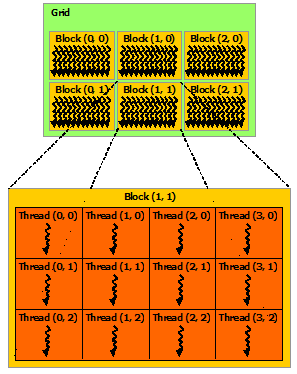
\includegraphics[width=0.5\linewidth]{0-resources/grid-of-thread-blocks}}\hspace{1em}%
	\subcaptionbox{\label{fig:blocks:b}}{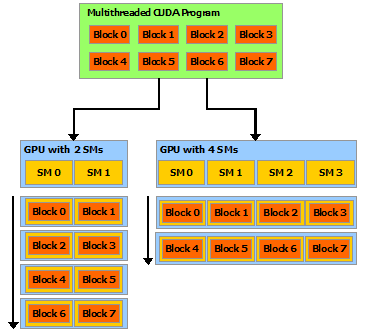
\includegraphics[width=0.7\linewidth]{0-resources/automatic-scalability}}
	\caption{(a): Grid of Thread Blocks; (b) Automatic Scalability. Those images was reprinted from \cite{cuda_manual} }
\end{figure}\\
As mentioned above, each block is assigned to a different streaming multiprocessor. On current GPUs, a block has a threads limit set to 1024, due to the limited memory resources of the SM. This block scheme is used to implement automatic scalability: indeed, the GPU schedules each block on any available SM, in any order. For example, if we have a program that divides the threads into eight blocks, it can be executed from both two GPU's with respectively two and four SMs without any intervention on the scheduling from the developer (Figure \ref{fig:blocks:b}).
\begin{figure}[h]
	\centering
	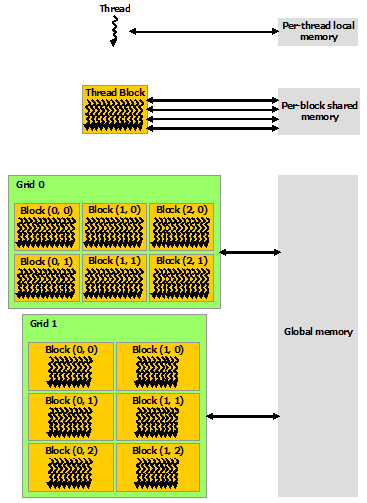
\includegraphics[width=0.6\linewidth]{0-resources/memory-hierarchy}
	\caption{Memory Hierarchy. This image was reprinted from \cite{cuda_manual}.}
	\label{fig:memory-hierarchy}
\end{figure}
On the other hand, the block schema allows also threads collaboration: as illustrated in the Figure \ref{fig:memory-hierarchy}, thanks to the allocation of each block to the same SM, allows those threads to share a fast per-block memory. Besides, all threads share the global device memory, even if they belong to different blocks or kernel (some advanced settings permit to execute two kernels simultaneously if there are enough resources. Those settings are not presented here because they are not used in this thesis, because a large amount of data doesn't permit to parallelize those kernels; moreover, for the sake of completeness, they are well described in \cite{cuda_manual}). The data must be copied to this memory from the host before the kernel execution. Those two types of memory, combined with several primitives that synchronize thread at warp, block or device levels, permit threads collaboration. Those synchronizing function acting as a barrier: all threads in the specific level must wait for the others before any one is allowed to proceed. In addition, CUDA exposes some other primitives that allow atomic operations (like add or compare and swap operation): if multiple threads call one of those methods on a specific memory address, the access to it will be serialized. No information about the order of the operation will be given a priori.
In conclusion, we remark that every new hardware architecture could introduce new features that aren't supported by the old GPU. For this reason, CUDA uses the concept of Compute Capability to identify the features supported by the GPU hardware. Our project use a compute capabilities greater than 6.0 .

\subsection{Thrust Library}
To conclude this CUDA introduction, we present Thrust, a powerful library of parallel algorithms and data structures that are largely used in this thesis project. This C++ Standard Template-based library is included in the CUDA toolkit and provides a reach collection of data-parallel primitives (as transform, sort or reduce) that allows writing a high performing and readable code with minimal effort. This presentation is based on the Thrust section present in the CUDA manual \cite{cuda_manual}.\\
We start the presentation from the two vector containers, \verb|host_vector| and\\\verb|device_vector|. As their name says, they are arrays that are dynamically allocated respectively in the host and in the device memory. Like the \verb|std::vector|, they are generic containers, their elements are allocated in contiguous storage locations and they can dynamically change the size. Indeed, using the \verb|=| operator, we can copy a \verb|host_vector| in a \verb|device_vector| and vice-versa. 
Thrust also provides many useful parallel algorithms, implemented for both host and device, like:
\begin{itemize}
	\item Sort that performs the sorting of a vector. It is also present its "by key" version that sorts a vector of values using another vector as a key;
	\item Reduce that performs a reduction of a vector. It is also present its "by key" version that, given a vector of values and a vector of keys, performs a reduction of the values for each consecutive group of keys;
	\item Transform that applies a function to each element of the vector;
	\item Exclusive and Inclusive Scans that perform a prefix sum, respectively ignoring and considering the corresponding input operand in the partial sum.
\end{itemize}
In this thesis, we use only the device CUDA-based version of this algorithm.
The last useful feature that Thrust provides is the fancy iterators. These iterators are used to improve performance in various situations. The \verb|transform_iterator|, for example, were used to optimize the code performing the transformation during the execution of an algorithm. Another very useful iterator is the \verb|zip_iterator| that takes multiple input sequences and yields a sequence of tuples: in this way we can treat many vectors as a single one and perform more operations simultaneously.
